\documentclass[a4paper,11pt,oneside, titlepage]{article}
\author{Groep 13: Sibrand Staessens en Sibren Polders}
\title{Trimesteroverschrijdend Project: Curve Editor}
\date{Donderdag 22 mei, 2008}
\usepackage[dutch]{babel}
\usepackage{verbatim}
\usepackage{graphicx}
\usepackage[colorlinks,urlcolor=blue,filecolor=magenta]{hyperref}
\usepackage{url}
\parindent 0pt	
\hyphenation{Hermite deze Monitor-Pool}
\fontfamily{times}
\begin{document}
\maketitle \newpage
\tableofcontents \newpage
\section{Voorwoord}
Op welke manieren kan je een set van punten op een vloeiende wijze met elkaar verbinden en hoe ziet het bekomen pad er dan uit ? Dat is
de vraag waarvoor Curve Editor een gedeeltelijke oplossing biedt. Het meest voor de hand liggende pad dat tussen de punten getekend kan worden 
is uiteraard dat pad dat bekomen wordt m.b.v. lineaire interpolatie. Maar er zijn nog zoveel andere mogelijkheden, waarvan er in Curve Editor twee verwerkt 
zijn (nl. Bézier- en Hermite-curves). Deze algoritmes zullen in vgl. met lineaire interpolatie vloeiende krommen
tussen de interpolatiepunten cre\"eren. De toepassingen van de door Curve Editor gebruikte algoritmes beperken zich niet enkel 
tot het tekenen van ``lijntjes'' tussen punten, maar worden bijvoorbeeld ook veelvuldig gebruikt voor vloeiende camerabewegingen of ``AI''-bewegingen in games.
De interpolatie van een gegeven set van controlepunten is een uitgebreide en interessante studie die 
op vele vlakken in de informatica/wiskunde zijn nut kan bewijzen. Curve Editor geeft er de 
basistoepassing van, namelijk die van de wiskundige berekening en grafische voorstelling van de gevraagde curve. \newline \newline \newline \newline
\newline \newline \newline \newline
%\begin{center}
%\textit{``If the path be beautiful, let us not ask where it leads.''} - Anatole France \newpage
%\end{center}
\newpage
\section{Wiskundige voorkennis \label{wv}}
\subsection{Lineaire interpolatie}
\subsubsection{Na\"ieve poging (brute force)}
Een eerste poging om een lineaire interpolatie te berekenen is die waarbij tussen elk paar van controlepunten
de vergelijking \begin{math}y = mx + b\end{math} wordt uitgerekend.
Hierbij geldt: \begin{math}m = (y_1-y_0)/(x_1-x_0)\end{math}, en b is het
startpunt op de y-as. De grote nadelen van dit algoritme zijn dat er voor iedere nieuwe
pixel opnieuw berekend en getekend moet worden en dat er behoefte is aan een floating-point optelling en 
vermenigvuldiging (vermits m een floating-point getal is).
\subsubsection{DDA-interpolatie (Digital Differential Analyzer)}
Bij deze methode wordt nog steeds m als een floating-point getal voorgesteld, maar de berekening van
de volgende y-waarde wordt als volgt vereenvoudigd:
\begin{math}
y_{i+1} = m.x_{i+1} + b\newline
= m.(x_i + \Delta x) + b\newline
= m.x_i + m.\Delta x + b\newline
= y_i + m.\Delta x\newline
= y_i + m \textrm{ aangezien } \Delta x = 1 \textrm{ als we 1 pixel verder gaan.} \newline
\end{math}
Dit algoritme is duidelijk effici\"enter vermits we geen floating-point vermenigvuldiging hebben 
verwijderd. 
\subsection{B\'ezier}
Het cubic Bézier-algoritme construeert een curve als volgt: per vier opeenvolgende controlepunten wordt een deel van de totale curve berekend.
Die deelcurve start in het eerste controlepunt, in de richting van het tweede, om dan in het vierde controlepunt te eindigen in de richting van het derde. Een volgende 
deelcurve heeft als eerste controlepunt het laatste controlepunt van de vorige deelcurve om alzo C0-continu\"iteit te garanderen.
\subsubsection{Na\"ieve poging (brute force)}
Bij een eerste poging kunnen we het algoritme implementeren a.h.v. de meetkundige constructie en de parametrische voorstelling van de curve.
Deze is als volgt:\newline
\begin{center}
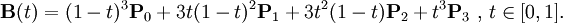
\includegraphics[scale=0.5]{bezier.png}
\end{center}
Indien we nu voor een eindig aantal t-waarden tussen 0 en 1, de B-waarde berekenen, dan hebben we een eindig aantal punten berekend die op de gevraagde curve
liggen. Gebruiken we nadien lineaire interpolatie om de berekende punten met elkaar te verbinden, dan hebben een eerste benadering van de cubic B\'ezier-curve.
Het spreekt voor zich dat deze implementatie verre van effici\"ent is: voor elke t-waarde moeten we de machten uitrekenen, vermenigvuldigen met de co\"ordinaten van de controlepunten
en daarna alles optellen. Dit is tijdsintensief rekenwerk, daarom is in Curve Editor het incrementeel aloritme, dat in de volgende sectie besproken wordt, ge\"implementeerd.
\subsubsection{Forward differences}
Deze implementatie is een incrementeel algoritme: de volgende berekening wordt gedaan a.h.v. wat in de vorige berekening werd gevonden. Op deze manier moet men voor elk gevraagd punt niet
helemaal van nul beginnen en minder rekenwerk uitvoeren. Hoe we tot de implementatie komen, gebeurt als volgt:

We evalueren de polynoom in een aantal even ver van elkaar liggende punten. Stel dat we $f(t) = a t^3 + b t^2 + c t + d$ willen evalueren voor de punten $t_0, t_1, ... , t_m$ met $t_{i+1} = t_i + \epsilon$ voor $i = 0, 1, ..., m-1$. Dan bekomen we:
\begin{center}
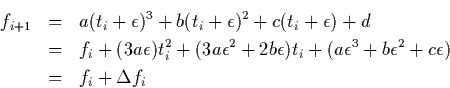
\includegraphics[scale=0.6]{diff1.png}
\end{center}
We noemen $\Delta f_i$ de voorwaartse differentie. Mer op dat $\Delta f_i$ een 2e-graadspolynoom is, een graad lager dan de originele polynoom. We passen hetzelfde toe voor $\Delta f_i$:
\begin{center}
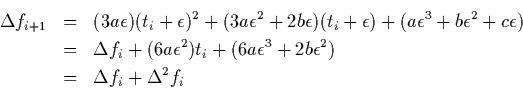
\includegraphics[scale=0.6]{diff2.png}
\end{center}
En voor $\Delta^2 f_i$:
\begin{center}
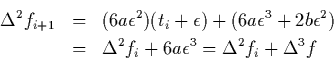
\includegraphics[scale=0.6]{diff3.png}
\end{center}
Samengevat hebben we dus:
\begin{center}
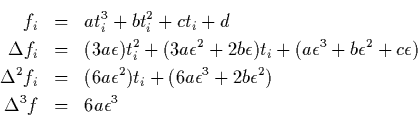
\includegraphics[scale=0.6]{diff4.png}
\end{center}
We moeten de startwaarden berekenen m.b.v. $t_0 = 0$:
\begin{center}
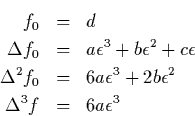
\includegraphics[scale=0.6]{diff5.png}
\end{center}
Nu hebben we alles wat we nodig hebben, en kunnen we de interpolatiepunten z\'elf gaan berekenen als volgt:
\begin{center}
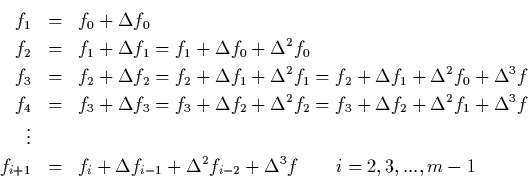
\includegraphics[scale=0.6]{diff6.png}
\end{center}
\subsubsection{C0-continu\"iteit}
C0-continue curves zijn de standaard curves, vermits C0-continu\"iteit enkel de eis oplegt dat de curve ononderbroken moet zijn.
Indien we als eerste controlepunt van een viertal het laatste controlepunt van het vorige viertal nemen, dan bekomen we automatisch C0-continu\"iteit. Deze eis vraagt dus geen veranderingen aan de controlepunten: het primitieve
B\'ezier-algoritme voldoet.
\subsubsection{G1-continu\"iteit}
G1-continu\"iteit eist dat de curves naast ononderbroken ook overal vloeiend ogen. Dit wordt dus bekomen door in elk controlepunt dat op de curve komt te liggen, de curve z\'o te berekenen dat de ingaande en de uitgaande raakvector
in dat controlepunt op \'e\'en lijn liggen. In Curve Editor is dit opgelost als volgt:

De ligging van het tweede en het derde controlepunt van een viertal B\'ezier-controlepunten wordt herberekend, zodanig dat de berekende curve vloeiend aansluit op de berekende curve voor het vorige en het volgende viertal. Stel het viertal v1 en viertal v2 opeenvolgende viertallen van controlepunten. Het laatste controlepunt van v1 en het eerste controlepunt van v2 zijn logischerwijs dezelfde: anders zouden we niet tot een aaneengesloten curve kunnen komen (zie C0-continu\"iteit). M.b.v. het voorlaatste controlepunt van v1, het gemeenschappelijke controlepunt en het tweede controlepunt van v2 berekent Curve Editor nu een nieuw voorlaatste controlepunt voor v1 en een nieuw tweede controlepunt voor v2 (het gemeenschappelijke blijft ongewijzigd). Dit doet het door de vector tussen het voorlaatste controlepunt van v1 en het tweede controlepunt van v2 te beschouwen; die vector wordt dan zodanig verschoven dat het gemeenschappelijke controlepunt op die vector komt te liggen. De twee uiteinden van deze verschoven vector zijn dan het nieuwe voorlaatste controlepunt voor v1 en het nieuwe tweede controlepunt voor v2. Indien we nu op die manier voor elk gemeenschappelijk controlepunt twee nieuwe controlepunten berekenen, dan bekomen we een mooi vloeiende curve.
\subsubsection{C1-continu\"iteit}
C1-continu\"iteit eist dat de curves naast ononderbroken zijn en overal vloeiend ogen, ook nog eens in elk controlepunt een gelijkmatig toe- en afnemende kromming hebben. Dit wordt dus bekomen door in elk controlepunt dat op de curve komt te liggen, de curve z\'o te berekenen dat de ingaande en de uitgaande raakvector
in dat controlepunt op \'e\'en lijn liggen \'en even groot zijn. In Curve Editor is dit opgelost als volgt:

De ligging van het tweede en het derde controlepunt van een viertal B\'ezier-controlepunten wordt herberekend, zodanig dat de berekende curve vloeiend aansluit op de berekende curve voor het vorige en het volgende viertal \'en zodanig dat de berekende curve een controlepunt even snel "binnenkomt" als "verlaat", met dezelfde versnelling als het ware. Stel het viertal v1 en viertal v2 opeenvolgende viertallen van controlepunten. Het laatste controlepunt van v1 en het eerste controlepunt van v2 zijn logischerwijs dezelfde: anders zouden we niet tot een aaneengesloten curve kunnen komen (zie C0-continu\"iteit). M.b.v. het voorlaatste controlepunt van v1, het gemeenschappelijke controlepunt en het tweede controlepunt van v2 berekent Curve Editor nu een nieuw voorlaatste controlepunt voor v1 en een nieuw tweede controlepunt voor v2 (het gemeenschappelijke blijft ongewijzigd). Dit doet het door de vector tussen het voorlaatste controlepunt van v1 en het tweede controlepunt van v2 te beschouwen; die vector wordt dan zodanig verschoven dat het gemeenschappelijke controlepunt midden op die vector komt te liggen. De twee uiteinden van deze verschoven vector zijn dan het nieuwe voorlaatste controlepunt voor v1 en het nieuwe tweede controlepunt voor v2. Indien we nu op die manier voor elk gemeenschappelijk controlepunt twee nieuwe controlepunten berekenen, dan bekomen we een mooi vloeiende en een in elk controlepunt even snel ingaand als uitgaand versnellende curve.
\subsection{Hermite}
\newpage
\section{Implementatie}
\subsection{Packages}
\subsubsection{Java packages}
Een Java package is een mechanisme binnen Java om klassen te organiseren in namespaces. 
Java broncode die binnen eenzelfde categorie of functie vallen kunnen hierdoor gegroepeerd 
worden. Dit kan door middel van een package statement bovenaan het beginbestand om aan te 
geven waartoe ze behoren. Dit is omwille van twee redenen handig: de klassen zijn dan gegroepeerd
in functionele categorie\"en, wat het geheel overzichtelijker maakt. En verder kunnen er nu twee 
verschillende klassen \'e\'enzelfde naam krijgen en toch uniek bepaald worden door er zijn
package name voor te zetten. Dit is zeker handig als de programmeur een klasse dezelfde naam
heeft gegeven als een klasse uit een library die hij wilt gaan gebruiken.\newline \newline
Voor Curve Editor zijn verschillende packages gemaakt, die zijn te zien op figuur \ref{packages}.
In wat volgt wordt een korte beschrijving gegeven van al deze packages, zonder \'al teveel op de technische details in
te gaan.
\subsubsection{CurveEditor}
Dit is wellicht de kleinste package van de reeks. Het bevat slechts \'e\'en klasse, 
namelijk die klasse die de main-methode bevat. Deze klasse zal, zoals wellicht duidelijk is, als bootstrap dienen voor Curve Editor. 
Er wordt ook de mogelijkheid geboden om rechtstreeks vanuit
de command line een bestand mee te geven. Dit is enkel ter volledigheid, vermits de gebruiker in de applicatie zelf zeer makkelijk bestanden kan inladen en opslaan.
\subsubsection{Algorithms}
Dit pakket voorziet de verschillende klassen die voor de interpolatiealgoritmen zullen zorgen.
Elke klasse in dit pakket implementeert de Algorithm-interface. Dit is handig voor latere uitbreidingen en groepswerk: deze interface 
legt immers vast welke functies de programmeur zal moeten implementeren, die functies worden immers elders in de applicatie gebruikt. \newline
De klassenamen zijn triviaal gekozen: ``Lineair, Bezier, BezierC1, BezierG1, Hermite, 
HermiteCardinal, HermiteCatmullRom''(zie figuur \ref{algorithms}). 
Zoals de namen al doen vermoeden, zullen deze klassen de verschillende
interpolatiemethodes besproken in het deel 'Wiskundige voorkennis' (\ref{wv}) implementeren.
Hierbij werd natuurlijk altijd geopteerd voor de meest optimale implementatie van degene die 
besproken werden.
\subsubsection{Core}
\label{tcore}
Dit pakket bevat enkele noodzakelijk klassen (zie figuur \ref{core}).\newline \newline
De klasse CurveContainer zal ervoor zorgen dat ingegeven punten kunnen opgeslagen worden, samen
met hun door interpolatie berekende punten. \newline \newline
Een eerste implementatie gebruikte het subdivision principe. In de beginsituatie is het tekenveld
dan \'e\'en grote rechthoek. Van zodra de gebruiker een curve begint te tekenen worden de secties,
waar nieuwe punten geplaatst zijn, onderverdeeld in steeds kleiner wordende rechthoekjes. In elk zo'n
rechthoekje zat dan juist \'e\'en punt van een curve. Nagaan welke curve op een bepaalde pixel lag, was op deze manier
makkelijk te achterhalen m.b.v. een quadtree.\newline
Deze implementatie bleek echter niet zo effici\"ent te zijn wanneer we te maken hadden met een groot
aantal controlepunten. Dit kwam voornamelijk doordat er telkens opnieuw kleinere rechthoekjes
moesten aangemaakt worden bij het ingeven van een nieuw punt, en een grotere wanneer er punten verwijderd
werden. Uiteindelijk was de applicatie meer bezig met het bepalen van rechthoekjes dan met zijn
doel: bijhouden en picken van curves. De gebruike datastructuur gaf wel mooie resultaten voor het zoeken van curves a.h.v.
een geklikt of gehooverd punt, maar wanneer de gebruiker de curves ging aanpassen (nieuwe punten, verplaatsen, connecteren, \ldots), dan ging de 
herberekening en aanpassing van de datastructuur echter tergend langzaam. Wij achtten het dan ook noodzakelijk dat we een andere manier
zouden vinden, die een betere balans tussen "aanpassen" en "informatie halen uit". \newline \newline
De tweede door ons ge\"implementeerde datastructuur leek ons direct bruikbaarder. Het aanpassen van de datastructuur ging immers direct een pak sneller in vgl.
met de vorige implementatie, de gebruiker kan nu bvb. redelijk vlug nieuwe controlepunten vlak achter elkaar ingeven. Ook het halen van informatie uit de datastructuur heeft een aanvaardbare snelheid.
Wat stelt die datastructuur nu precies voor ? We stellen een tweedimensionale matrix op waarvan elk element een referentie kan bevatten naar een curve-instantie.
Het toevoegen van curves is op deze manier zeer simpel te doen: voor elk punt van de curve plaatsen we in de overeenkomstige cel van de matrix een referentie naar de curve.
Curves verwijderen is dan gewoon het tegenovergestelde: al die cellen weer naar null laten wijzen. Het zoeken naar een curve a.h.v. een punt (a.h.v. co\"ordinaten van een muisevent, bijvoorbeeld) 
gaat nog vrij snel omdat we enkel maar in een bepaalde range in de matrix de inhoud van de cellen moeten bekijken. Indien een niet-null referentie in die range aanwezig is, dan weten we welke curve
daar ligt.\newline \newline
De klasse Editor is het hart van Curve Editor. Deze zal zorgen dat gegevens tussen de verschillende datastructuren (Point, Curve, Algorithm) kan doorgegeven worden.
De uitwisseling van data zal voornamelijk bestaan uit het zoeken/verwijderen van punten uit de CurveContainer-klasse en het veranderen van Curves (verplaatsen, punten toevoegen/verwijderen, type veranderen, \ldots).
Maar ook het opvangen en afhandelen van excepties gebeurt grotendeels in Editor. Deze klasse zorgt er m.a.w. voor dat de 
verschillende andere klassen zo autonoom mogelijk kunnen werken, Editor is dan de klasse die alles samenbrengt. Dit verhoogt natuurlijk ook de leesbaarheid en onderhoudbaarheid van de code.\newline \newline
Een laatste klasse van dit pakket is de FileIO-klasse, deze zal niet alleen bestanden opslaan en
inladen, maar ook zal hij de undo/redo-functionaliteit, vermits deze van
dezelfde functies gebruik maakt. Er wordt dan gewoon een stack van bestanden in het geheugen bijgehouden.
\subsubsection{Curves}
Dit pakket bevat de twee datatypes die doorheen het programma gebruikt worden. Point verzorgt, zoals
de naam doet vermoeden, de datastructuur die punten voorstelt. Curve geeft dan weer de
mogelijkheid om een verzameling van punten (lees: een kromme of curve) op te slaan. De
technische details van deze laatste klasse worden beter uitgelegd verder in de tekst (zie ). 
Voorlopig is het voldoende om te weten dat Curve een vector van Point-instanties bijhoudt en enkele
basisvoorzieningen voorziet (punten opvragen, toevoegen, transleren, \ldots).
\subsubsection{Exceptions}
Een foutloos programma schrijven is op zich al een opgave, vermits er altijd wel kleine bugs
kunnen opduiken na langdurig en gevari\"eerd gebruik. Foolproof code schrijven daarentegen is een
onmogelijke opgave. Daarom hebben we gebruik gemaakt van exceptions om ``verkeerd'' gebruik van
CurveEditor-functies op te vangen. Onder verkeerd gebruik valt bijvoorbeeld het inladen van een
onbestaande file of een verkeerd bestandsformaat, het toevoegen van een punt zonder er de 
co\"ordinaten van op te geven, \ldots. Maar ook met toekomstige uitbreidingen in gedachte zijn exceptions een handig middel,
niet elke programmeur hanteert immers dezelfde logica. Vindt de \'e\'en dat aan een methode bijvoorbeeld geen null-waarden kunnen worden meegegeven omdat 't nonsens lijkt, dan kan een ander vinden dat het wel mogelijk moet zijn om dat te doen. Exceptions laten die andere dan weten dat zo'n parameters nooit mogen meegegeven worden wil hij een resultaat verkrijgen, zonder dat hij naar de broncode van die ene methode hoeft te kijken.\newline \newline
Er zijn ook twee HandleException-klassen voorzien: eentje in dit pakket, deze zal gewoon 
het exceptie bericht in de console uitprinten, en eentje in het GUI-pakket, die in een dialoogvenstertje de exceptie zal uitprinten.
\subsubsection{GUI}
De GUI is vrij grondig opgesplitst (zie figuur \ref{gui}). Elk groot deel heeft zo zijn eigen klasse; 
zo heb je een menubalk-klasse, een snelknopbalk-klasse, een tekengebied-klasse en een keuzegebied-klasse. \newline
De GUI-klasse zal op zijn beurt het centrale orgaan spelen die al deze klassen met elkaar verbindt.
Het is daarom ook logisch dat deze is afgeleid van de klasse Editor,
de centrale klasse van de Core-package. Zo kunnen immers Core-functionaliteiten aan GUI-events e.d. gelinkt worden.
\newline
Het opdelen van de GUI in verschillende klassen heeft enorme voordelen als we spreken 
over leesbaarheid en onderhoudbaarheid van code. Het EventHandling-systeem van Java zelf is overigens
optimaal voor dit soort afscheiding. In Java worden de events immers opgevangen in een klasse,
die afgeleid wordt van een van de Listener-interfaces (ActionListener, ItemListener, \ldots). Deze 
klasse zal dan de door de interface opgelegde functies impementeren om alzo de juiste evenafhandeling te kunnen
doen. Het is dus voldoende om deze EventHandling-klassen in GUI aan te maken en door te geven
aan de juiste componenten (menubalk, tekengebied, \ldots). Meer uitleg hierover vind je verder in
de tekst.
\subsubsection{Tools}
Dit bevat een curvesimulator. In principe is het een ``chique'' naam voor een bolletje
dat over het pad dat de curve voorstelt loopt. Dit kan bijvoorbeeld door de gebruiker gebruikt worden om de stijging en daling
van de curve te bestuderen. Zodoende kan hij de getekende curve visueel evalueren.
\subsection{Uitwerking van de GUI}
\subsubsection{Overzicht}
Zoals in screenshot \ref{scr_gui} te zien is kan de vormgeving van de GUI in 4 grote stukken worden opgedeeld:
\begin{enumerate}
\item Menubalk
Hierin kan de gebruiker elke actie terugvinden die door Curve Editor kan gedaan worden.
Bijna elke actie is ook aan te roepen met behulp van sneltoetscombinaties ( Alt-F, Ctrl-O, \ldots ), zodat
elke gebruiker op zijn favoriete manier kan navigeren doorheen de verschillende uitvoerbare taken.
Er is overigens aandacht geschonken aan de nesting van de menu-items: die mogen niet te diep noch te breed zijn.
Verder is elke naam zo triviaal mogelijk gekozen en meestal wordt die ook voorzien van een icoontje.
\item Snelknopbalk
Hierin vind je enkele veelgebruikte taken terug (nieuw bestand beginnen, bestand openen, 
nieuwe curve starten, \ldots). Dit is voorzien opdat de gebruiker deze taken snel en en dus effici\"enter kan
afhandelen dan wanneer hij dat telkens vanuit de menubalk zou moeten doen.
\item Keuzegebied
In dit gebied zal de gebruiker snel kunnen kiezen welk type curve hij wilt tekenen (B\'ezier, 
Hermite, \ldots) en kan hij ten alle tijden een punt aan de op dat moment geselecteerde curves toevoegen door 
de co\"ordinaten in te geven. Verder kan de gebruiker hier ook kiezen of hij de co\"ordinaten, raakvectoren en 
puntnummers van de geselecteerde curves wilt laten uittekenen. \newline
Het Edit-veld van dit gebied hangt af van de mode waarin je bezig bent. Er zijn voor de gebruiker
twee grote modi "voelbaar". De eerste is curve-modus: hier bewerk je de curves op zich (selecteren, 
deselecteren, nieuwe curve maken, \ldots); de tweede is controlepunt-modus (punt verslepen, selecteren, toevoegen).
Naargelang de modus waarin je zit zullen andere mogelijkheden zichtbaar worden in het Edit-veld.
Dit leidt tot een groter gebruiksgemak vermits de taken die verschijnen meestal ook gebruikt
worden wanneer je in die modus werkt.
\item Tekengebied
Dit gebied is waarschijnlijk wel het interessantste voor de gebruiker. Met behulp van muisinteractie
kan de gebruiker controlepunten aan dit veld toevoegen en deze punten laten connecteren
door een interpolatiealgoritme. De gebruiker kan tevens in dit veld punten en curves selecteren,
verwijderen en zelfs verslepen. Het tekengebied maakt gebruik van double buffering om 
beeldflikkering te vermijden en ook van clipping zodat alleen getekend wordt wat ook echt
op het scherm k\'an verschijnen.
\end{enumerate}
\subsection{Listeners in Java}
Java heeft een aparte stijl om events op te vangen (signalen gestuurd door buttons, menu-items,
\ldots). De taal bezit hiervoor zogenaamde EventListener-interfaces. De programmeur
moet een klasse aanmaken die een dergelijke interface zal implementeren. Deze klasse wordt dan
m.b.v. een simpel commando geconnecteerd met een bepaalde component (bijvoorbeeld een button).
In de interface is er een EventHandle-functie gedefini\"eerd die door de programmeur zal 
ge\"implementeerd worden, zodat, wanneer de component een event genereert,
die opgevangen en afgehandeld kan worden.\newline

Dit systeem is pas echt voordelig als je een event moet afhandelen in een geneste klassestructuur. 
Stel als voorbeeld: je hebt in een klasse A een instantie van een klasse B zitten
die op zijn beurt dan weer een instantie heeft van klasse C, en je wilt dat klasse A een handeling
doet als klasse C een event uitstuurt.
Met callbacks is de properste manier (om klasse-onafhankelijkheid te bewaren) een callback 
te connecteren van klasse A naar klasse B en daarna een callback van klasse B naar klasse C.
In Java kan je gewoon een EventHandle-klasse vanuit klasse A meegeven aan B die het op zijn 
beurt meegeeft aan klasse C. Dit maakt de structuur natuurlijk wat eenvoudiger, overzichtelijker, en makkelijker te begrijpen.\newline \newline

In deze implementatie is ervoor gekozen om deze EventHandle-klassen in de klasse GUI te 
defini\"eren. Het voordeel hiervan is dat enkel de klasse GUI de EventHandle-klassen kan 
instanti\"eren en deze instanties zullen alle membervariabelen en -functies van GUI zelf kunnen 
gebruiken. Dit zorgt ervoor dat er geen extra connectie moet gelegd worden tussen de 
EventHandle-klassen en GUI. Je kan dit dus bekijken als een soort van friendly class die niet ge\"instantieerd kan worden.
\subsection{Datastructuren}
\subsubsection{Point}
Deze datastructuur heeft niet zoveel uitleg nodig, een Point bestaat namelijk uit zijn x- en y-waarde en is daarmee
volledig gedefini\"eerd. De nodige get()- en set()-functies zijn ook voorzien, uiteraard.
\subsubsection{Curve}
Deze structuur heeft al iets meer uitleg nodig. Een curve is, vanuit het laagste niveau bekeken, niets 
anders dan een container van zijn punten.\newline
Elke Curve houdt drie essenti\"ele dingen bij
\begin{enumerate}
\item zijn type (B\'ezier, Hermite, \ldots)
\item een Vector van controlepunten: deze wordt dus gevuld wanneer de gebruiker een nieuw controlepunt aan de curve toevoegt
\item een Vector van outputpunten: deze wordt a.h.v. de Vector van controlepunten en m.b.v. een Algorithm-instantie gevuld
\end{enumerate}

Hierbij worden het type en de controlepunten dus door de gebruiker ingegeven/veranderd. De vector van outputpunten
wordt intern berekend door de verschillende interpolatiealgoritmen. Het aanroepen van deze Algorithm-functies gebeurt niet in Curve, maar in Editor, de klasse die alle datastructuren samenbrengt.
De vectoren worden ook door de GUI gebruikt om de curve op het tekengebied te kunnen uittekenen.\newline

Om de punten op te slaan hebben we voor een Vector gekozen, omdat de verschillende
interpolatietechnieken gemakkelijk moeten kunnen "springen" tussen de gegeven controlepunten om
hun algoritme te kunnen uitvoeren.

Deze klasse bevat ook nog functies om punten te verwijderen, toe te voegen, om na te gaan of een gegeven punt al dan niet tot de curve behoort, \ldots.
\subsection{Extra's}
Echte extra's hebben we niet ge\"implementeerd, onderstaande uitgezonderd. Bestanden opslaan naar meerdere formaten (*.xml en *.gif/*.png), bestanden inladen, oneindige undo/redo-stack, meer performante code verkiezen, selectietooltje m.b.v. dragging, \ldots beschouwen we gewoon als "nodig" voor Curve Editor.
\subsubsection{Path Simulation Tool}
Dit tooltje loopt de geselecteerde curves \'e\'en voor \'e\'en af, en laat een bolletje verschijnen dat als het ware "loopt" van het begin naar het einde van de curve. Het starten van deze tool, laat een nieuwe thread starten, zodat men \'en de tool kan laten runnen \'en men terwijl de geselecteerde curves zelf nog kan aanpassen (verslepen e.d.). 
\subsection{Interessante problemen}
\subsubsection{Vector vs. LinkedList}
Hoewel de collecties van outputpunten van curves enkel maar sequentiëel worden doorlopen (toevoegen achteraan, hele inhoud verwijderen, van voor naar achter uittekenen, \ldots), bleek Vector toch de betere keuze te zijn.
Hoewel de structuur van LinkedList ook zou moeten voldoen, maar met een kleiner geheugenverbruik dan Vector, bleek deze datastructuur tergend langzaam te werken. Een reden hiervoor hebben we niet gevonden, maar door gewoon terug gebruik te maken van Vector was het probleem ook opgelost.
\subsubsection{HashMap vs.2D Matrix}
Voor de CurveContainer, die de picking moet afhandelen, hadden wij aanvankelijk een HashMap gebruikt. De keys van de HashMap in de bovenste laag waren de pixels/punten van het scherm, en de values waren referenties naar rechthoekjes. Bij initialisatie van de CurveContainer wijzen alle values naar eenzelfde rechthoek. Elk van die rechthoekjes bevat \'e\'en referentie naar een Curve-instantie en een Point-instantie, of twee null-referenties. Zo wordt elk rechthoekje gemapt op een Curve.

Wordt er een extra punt aan de container toegevoegd, dan wordt de rechthoek naarwaar de pixel momenteel verwijst opgesplitst in vier deelrechthoekjes, indien die niet naar null verwijst en indien de resulterende rechthoekjes niet t\'e klein zijn. Indien die wel naar null refereert, dan wordt de hele rechthoek gemapt op die Curve zonder de rechthoek daarvoor op te splitsen, en wordt de Point-referentie gelijkgesteld aan de referentie naar het nieuwe controlepunt. Als er vier deelrechthoekjes aangemaakt dienen te worden, dan wordt voor elk van die rechthoekjes bepaald naar welke Curve zij moeten verwijzen, die van het nieuwe controlepunt, of de Curve waarnaar de grote rechthoek refereerde. Het rechthoekje waarin het nieuwe controlepunt ligt, wordt automatisch aangepast zodat het naar de andere Curve verwijst. Voor de 3 andere wordt de afstand berekend van het middelpunt van het rechthoekje tot het punt naarwaar de Point-instantie van de omkoepelende rechthoek wijst. Is die afstand groter dan de afstand van het middelpunt tot het nieuwe controlepunt, dan zal dat rechthoekje niet de referenties van de omkoepelende rechthoek overnemen, maar naar de nieuwe Curve/Point refereren.
Alle punten in dat rechthoekje wijzen in de HashMap naar dat rechthoekje, uiteraard.

Een curve verwijderen gaat als volgt: men gaat voor alle punten de hashmap af, indien het gevonden rechthoekje naar de curve wijst, dan dient dat rechthoekje aangepast te worden. Als de omliggende rechthoekjes naar eenzelfde curve verwijzen, dan wordt van die vier rechthoekjes weer één rechthoek gemaakt. Indien de omliggende rechthoekjes niet naar eenzelfde curve verwijzen, dan wordt weer de afstand berekend van het middelpunt van het te veranderen rechthoekje tot de punten naarwaar de andere rechthoekjes refereren. Hetgeen de kleinste afstand oplevert, heeft de referenties die men zoekt. 

Een Curve opzoeken gaat razendsnel doordat gewoon in de bovenste HashMap de value voor de key/punt gehaald moet worden. 
A.h.v. het bekomen rechthoekje kan men weten naar welke Curve het punt wijst.

Jammer genoeg ging het telkens aanpassen van de hele rechthoekstructuur zeer langzaam wat tot ergernissen bij de eindgebruiker zou leiden. Het picken ging echter wel h\'e\'el vlug, maar we verkiezen toch een datastructuur die misschien net iets minder vlug is voor picking, maar voor aanpassingen aanvaardbare snelheden geeft.
Een eerste datastructuur die we implementeerden was een simpele Matrix zoals die uitgelegd werd in sectie \ref{tcore}. Die bleek vlot genoeg te werken, dus uiteindelijk hebben we deze datastructuur maar behouden.
\subsubsection{Systeemafhankelijke problemen}
Op de meeste PC's werkt Curve Editor zoals het hoort, maar op sommige systemen blijkt het toch minder performant te werken.

Zo werkt het pixel-tekenen van Curve-Editor op UHasselt-laptops z\'e\'er traag. Dit zal waarschijnlijk te wijten zijn aan slechte Nvidia-drivers, want op diezelfde laptops werkt het in Linux wel vlotjes.
Op andere geteste Windows-systemen doken er geen problemen op.

Een foute configuratie van de Xorg-server in Linux zorgt ook voor problemen. Zo is het op \'e\'en getest systeem onmogelijk Curve Editor te resizen of te verplaatsen. Dat laatste lukt wel, maar het zorgt ervoor dat 
wanneer je dan op menu-items klikt, ze direct terug "wegspringen".
\newpage
\section{Planning}
\newpage
\section{Taakverdeling}
\begin{enumerate}
\item Sibrand Staessens:
       Bezier algorithmes, CurveContainer, Editor, DrawArea, GUI
\item Sibren Polders
       Hermite algorithmes, FileIO, Menu, ToolBar, ChoiceArea, GUI, PathSimulation
\end{enumerate}
\newpage
\section{Appendix}
\appendix
\section{Handleiding}
Had gij dacht ik?
\section{Screenshot}
Gij ook? Alleja ik ga kijken welke gij al hebt en dan bijmaken wat ik nodig heb. Zodoende gaan
we geen dubbel werk leveren \ldots. ``Stel niet uit tot morgen wat je vandaag door een ander
kan laten doen''
\section{Referenties}
Prof. dr. F. VAN REETH, Prof. dr. P. BEKAERT, 2007-2008, Computer Graphics\newline
\url{http://en.wikipedia.org/wiki/Bezier\_curve} (Bezier)\newline
\url{http://home.scarlet.be/piet.verplancken3/bezier/node9.html} (B\'ezier)\newline
\url{http://en.wikipedia.org/wiki/Catmull-Rom\_spline} (Hermite)\newline
\url{http://java.sun.com/javase/6/docs/api/} (Java)\newline
\url{http://java.sun.com/docs/books/tutorial/uiswing/events/intro.html} (Event en Listeners)\newline
\url{http://www.w3schools.com/xml/default.asp} (XML)\newline
\url{http://www.w3schools.com/dtd/default.asp} (DTD)\newline
\url{http://www.totheriver.com/learn/xml/xmltutorial.html} (XML)\newline
\url{http://www.kde.org/} (icoontjes)\newline
\end{document}
